

\chapter{Basics of State Space}\label{BasicsStateSpaceChapter}


\section{Problem Statement and Learning Objectives}

Most of this course will cover control system design using system transfer functions (rational polynomials in $s$ which describe the input-output relationships of system blocks).  However when we write the equations of motion, it is an ideal time to introduce a couple of concepts from the ``modern control theory'' introduced in the 1960's which has supplanted the $s$ domain methods in some applications.

\paragraph{Learning Objectives}
Be able to
\begin{itemize}
    \item Understand the basic system equations to represent a linear
    dynamic system in state space.
    \item Convert equations of motion (EOMs) into state space
    representation.
    \item Use the computer to plot step response and state trajectories from
    the state space model.
\end{itemize}

\section{Introduction}\label{SSeomIntro}
In ``modern'' control theory, the system is represented as a first order linear differential equation in a high dimensional space known as state space.  Each point in state space represents a unique dynamical state of the system.   For example, a system with one mass could be described by a 2-dimensional state space consisting of the position, $x$ and the velocity, $\dot{x}$ (Figure \ref{2Dstatespace}). $x$ and
$\dot{x}$
are the variables in the equations of motion for the mass (we consider $\ddot{x}$
separately).

\begin{figure}\centering
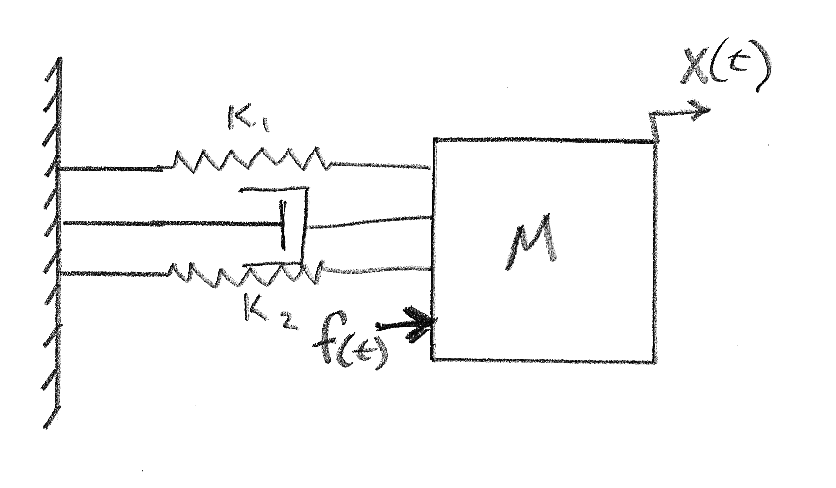
\includegraphics[width=65mm]{figs04/01069.png}   \hspace{0.25in}
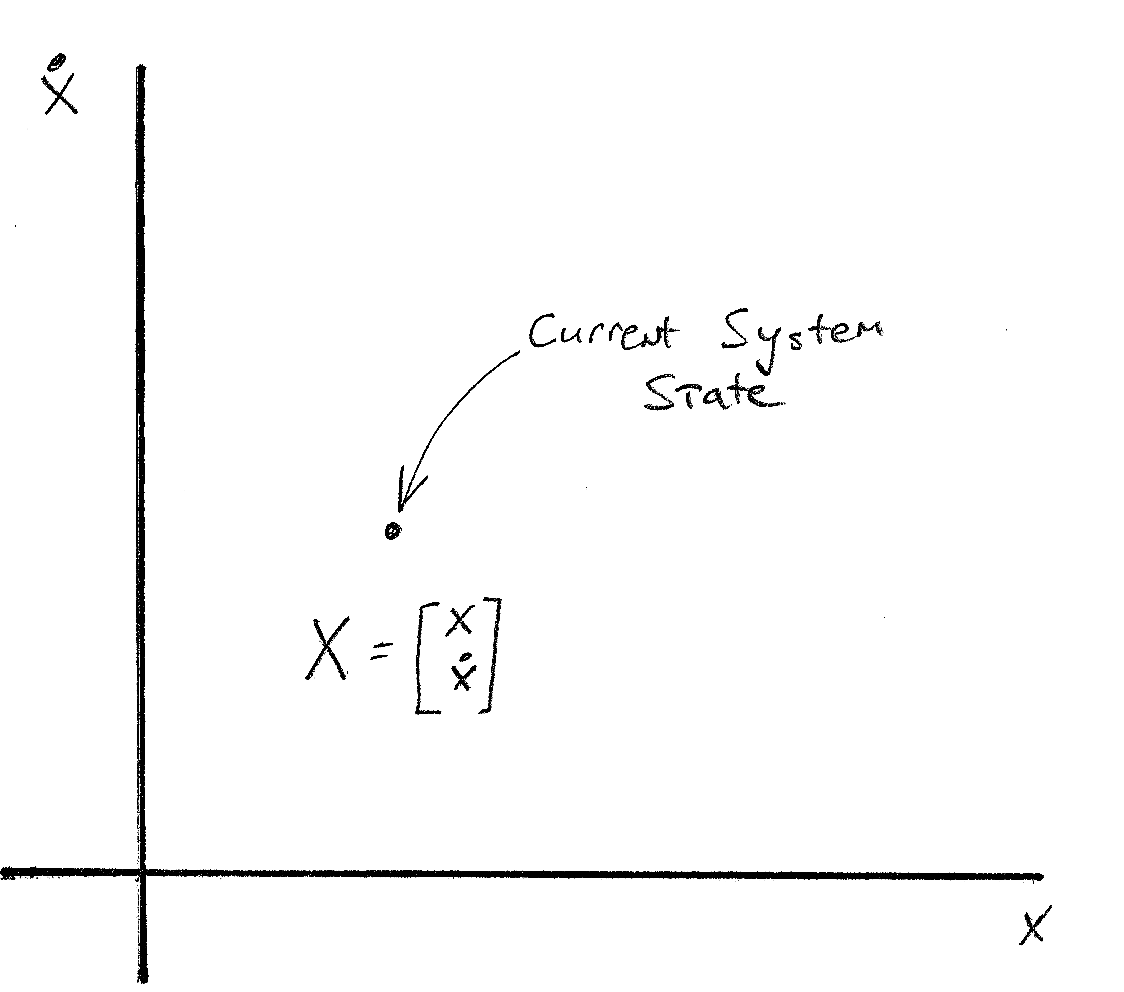
\includegraphics[width=45mm]{figs04/01075.png}
\caption{Translational dynamic system for state space example.}\label{2Dstatespace}
\end{figure}

The way to define the dimensionality of a system's state space is to identify all system variables which describe an energy.  Each one is a dimension of state space.   In our single mass example, energy is stored in the spring and mass:
\[
E_K = \frac{1}{2}(K_1 + K_2)x^2 \qquad E_M = \frac{1}{2}M{\dot{x}}^2
\]
So for this system we would use $x$ and $\dot{x}$ as state variables.
We use a vector, $X$, to define a point in state space such as:
\[
X = \begin{bmatrix} x \\ \dot{x} \end{bmatrix}
\]
Then the dynamics of the system are represented in a matrix first order LODE:
\[
\dot{X} = AX+BU
\]
Where $X$ is the state vector, $\dot{X}$ is the first derivative of the state vector,
\[
\dot{X} = \begin{bmatrix}\dot{x} \\ \ddot{x} \end{bmatrix}
\]
$A$ is a matrix of constant coefficients,
$U$ is the system input (like an applied force, $f(t)$), and
$B$ is another matrix.  This form can represent systems with multiple inputs (the elements of $U$), but here we will restrict ourselves to a single input
(see below).

Sometimes the output of the system, $Y$, is not one of the state variables, but instead a linear
combination of the state variables and possibly the input. For example, this could occur in
a blood pressure controller where states could be
blood volume, cardiac output, and vascular resistance, but  output, blood pressure,
is a linear combination of those states.
In this case there is another equation
\[
Y = CX+DU
\]
where $C,D$ are additional matrices of constant coefficients.
There is no Laplace transform and the
equations come directly from the equations of motion. In many realistic systems,
many  elements of these matrices are zero.

In this course, we focus on systems with a single input and single output (known as a
SISO system) and thus $u$ and $y$ are scalars and the matrices $B,C,D$ are not square.

\subsection{Dimensions of your State Equation Matrices}Source: \href{https://en.wikibooks.org/wiki/Control_Systems/State-Space_Equations}{WikiBooks Control Theory}

With the following notation, we easily define the dimensions of $A,B,C,D$.

\vspace{0.25in}
\noindent
Define $p,q,r$ as
\[
\begin{aligned}
    p &= \mathrm{number\; of\; states}\\
    q &= \mathrm{number\; of\; inputs} \\
    r &= \mathrm{number\; of\; outputs} \\
\end{aligned}
\]

Then the matrix dimensions are:

\begin{center}
  \begin{tabular}{c|c}
  Matrix & Dims \\\hline
     A  & $p\times p$ \\
     B  & $p\times q$ \\
     C  & $r\times p$ \\
     D  & $r\times q$ \\
  \end{tabular}
\end{center}



\section{System Matrices from Equations of Motion}\label{SecSystemMatricesFromEOMs}
Let's see how EOMs turn into the State Space representation using the example system of Figure \ref{2Dstatespace}.  Writing the EOM:
\[
M\ddot{x}+B\dot{x}+(K_1+K_2)x = f(t)
\]
rearranging to solve for $\ddot{x}$:
\[
\ddot{x} = \frac{1}{M}\left[ -B\dot{x}-(K_1+K_2)x+f(t)\right ]
\]
\[
\ddot{x} = -\frac{B}{M}\dot{x} - \frac{K_1+K_2}{M}x + \frac{1}{M}f(t)
\]
Converting this to a matrix equation is just rearranging according to
\[
       \dot{X} = \begin{bmatrix}\dot{x} \\ \ddot{x} \end{bmatrix}
\qquad      X  = \begin{bmatrix} x \\ \dot{x} \end{bmatrix}
\qquad U       = \begin{bmatrix}f(t)\end{bmatrix}
\]
%  \begin{bmatrix}\end{bmatrix}
then we have
\[
\dot{X} =
\begin{bmatrix}\dot{x} \\ \ddot{x} \end{bmatrix} =
\begin{bmatrix}0&1\\\frac{-(K_1+K_2)}{M}&\frac{-B}{M}\end{bmatrix}
\begin{bmatrix}x\\ \dot{x}\end{bmatrix}+
\begin{bmatrix}0\\ \frac{1}{M}\end{bmatrix}
\begin{bmatrix}f(t)\end{bmatrix}
\]
The top row is sort of a trivial equation, and the second row is the rearranged equation of motion.
This is the state space description for the system of Figure \ref{2Dstatespace}.


\begin{Example}\label{suspensionstatespace}
Consider the car suspension
Example 2.\ref{ExampleCarSuspension} and Example 2.\ref{ExampleCarSuspensionTF}.
\vspace{0.2in}
Derive the state space representation.

The EOMs were:
\begin{align*}
&M_w\ddot{x}_2+B_s(\dot{x}_2-\dot{x}_3)+K_s(x_2-x_3)+K_t(x_2-x_1) =0 \\
&M_v\ddot{x}_3+B_s(\dot{x}_3-\dot{x}_2)+K_s(x_3-x_2) = 0
\end{align*}
Note that the input to this system is $x_1$, the displacement of the road.  We  can
re-write the EOMS to put the input on the RHS:
\begin{align*}
&M_w\ddot{x}_2+B_s(\dot{x}_2-\dot{x}_3)+K_s(x_2-x_3)+K_tx_2 = K_tx_1 \\
&M_v\ddot{x}_3+B_s(\dot{x}_3-\dot{x}_2)+K_s(x_3-x_2) = 0
\end{align*}
Let the state vector be:
\[
X = \begin{bmatrix}x_2 & \dot{x}_2 & x_3 & \dot{x}_3\end{bmatrix}^T
\]
(where T indicates transpose to make $X$ a column vector)
and its derivative is
\[
\dot{X} = \begin{bmatrix}\dot{x}_2 & \ddot{x}_2 & \dot{x}_3 & \ddot{x}_3\end{bmatrix}^T
\]
Rearranging the EOMS:

\begin{align*}
\ddot{x}_2  &= \frac{1}{M_w}\left [-(K_T+K_s)x_2-B_s\dot{x}_2+K_sx_3+B_s\dot{x}_3\right]\quad+\quad \frac{1}{M_w}K_tx_1 \\
\ddot{x}_3 &= \frac{1}{M_v}\left[+K_sx_2+B_s\dot{x}_2 -K_sx_3-B_s\dot{x}_3\right]
\end{align*}
We will treat the variable $x_1$ in the $\ddot{x}_2$ EOM as our system input:
\[
U = \begin{bmatrix}x_1\end{bmatrix}
\]

We then have the 4x4 matrix state equations:
\[
\dot{X} = AX+BU
\]
\[
\dot{X} = \begin{bmatrix}\dot{x}_2 \\ \ddot{x}_2 \\ \dot{x}_3 \\ \ddot{x}_3\end{bmatrix}
=
\begin{bmatrix} 0&1&0&0\\
\frac{-(K_T+K_s)}{M_w}&\frac{-B_s}{M_w}&\frac{K_s}{M_w}&\frac{B_s}{M_w}\\
0&0&0&1 \\
\frac{K_s}{M_v}&\frac{B_s}{M_v}&\frac{-K_s}{M_v}&\frac{-B_s}{M_v}\\
\end{bmatrix}
\begin{bmatrix}x_2\\\dot{x}_2\\x_3\\\dot{x}_3 \end{bmatrix}+
\begin{bmatrix}
    0\\
    \frac{K_t}{M_w}\\
    0\\
    0\\
\end{bmatrix}
\begin{bmatrix}x_1\end{bmatrix}
\]

Where we have set the dimensions of $A,B$ according to the scheme above with

\[
\begin{aligned}
    p &= \mathrm{number\; of\; states} = 4\\
    q &= \mathrm{number\; of\; inputs} = 1\\
    r &= \mathrm{number\; of\; outputs} = 1 \\
\end{aligned}
\]

\end{Example}


\begin{ExampleCont}
You can verify that rows 2 and 4 of the matrix equation above are equivalent to the
two EOMS.   For example, row 2 is:
\[
\ddot{x}_{2} = \frac{-(K_T+K_s)}{M_w}x_2+\frac{-B_s}{M_w}\dot{x}_2+\frac{K_s}{M_w}x_3\frac{B_s}{M_w}\dot{x}_3
\]
Also note that we have two trivial equations: rows 1 and 3:
\[
\dot{x}_2 = \dot{x}_2 \qquad \dot{x}_3 = \dot{x}_3
\]
These are just part of the formal definition of the system matrices.
Once your parameter values are known, you can plug them in and it is easy to evaluate the response to any input using the computer.
As a formal matter, let's do an output equation.   Assume that for some reason our
system output is a mixture of the states, namely
\[
y(t) = 0.5x_2 + 0.01\dot{x}_3
\]
 then our output equation, $Y=CX+DU$ would be
\[
\begin{bmatrix}y(t)\end{bmatrix} =
[0.5, 0, 0, 0.01]X + [0] x_1
\]
(also following the $p,q,r$ dimensioning scheme).
$D$ is zero because we have no $x_1$ term in our output.  For most of our examples though,
the output equation will be trivial.  In this example, the output is $x_3(t)$ (car body height)
and thus
\[
\begin{bmatrix}y(t)\end{bmatrix} =
[0,0,1,0]X + [0] x_1
\]
\end{ExampleCont}

%
% To see that there are infinitely many SS representations of a linear system, consider a
% rotation matrix such as
% \[
% R = \begin{bmatrix}1 & \cos{\theta} \\ -\sin{\theta} & 1\end{bmatrix}
% \]
% (such a matrix is called ``orthonormal'' and has eigenvalues of unit magnitude).   The key point
% is that multiplying a matrix by a rotation matrix does not change its eigenvalues at all.   Therefore,
% if $R$ is orthonormal we can write
% \[
% RY = RAX+RBU
% \]
% and we have a new system matrix  $RA$ which represents the same system as $A$.
%



\subsection{Sources}
For Toyota Camry Suspension Parameters:
\begin{itemize}
    \item R.K. Taylor, L.L. Bashford, M.D. Schrock, ``Methods for Measuring Vertical Tire Stiffness,''
    Transactions of ASAE, vol 34, p 1415-1419, 2000
    \item M.D. Rao, S.Gruenberg, ``Measurement of Equivalent Stiffness and Damping of Shock Absorbers,''
    \item J. Iwaniec, ``Identification Of Car Suspension System Parameters On The Basis Of Exploitational Measurements,'' Diagnostyka, V14, N2, 2013
\end{itemize}

